\documentclass[10pt,]{article}
\usepackage{lmodern}
\usepackage{amssymb,amsmath}
\usepackage{ifxetex,ifluatex}
\usepackage{fixltx2e} % provides \textsubscript
\ifnum 0\ifxetex 1\fi\ifluatex 1\fi=0 % if pdftex
  \usepackage[T1]{fontenc}
  \usepackage[utf8]{inputenc}
\else % if luatex or xelatex
  \ifxetex
    \usepackage{mathspec}
  \else
    \usepackage{fontspec}
  \fi
  \defaultfontfeatures{Ligatures=TeX,Scale=MatchLowercase}
\fi
% use upquote if available, for straight quotes in verbatim environments
\IfFileExists{upquote.sty}{\usepackage{upquote}}{}
% use microtype if available
\IfFileExists{microtype.sty}{%
\usepackage{microtype}
\UseMicrotypeSet[protrusion]{basicmath} % disable protrusion for tt fonts
}{}
\usepackage[margin=1.0in]{geometry}
\usepackage{hyperref}
\hypersetup{unicode=true,
            pdftitle={Department Invited Speakers Do Not Reflect Trainee Diversity},
            pdfborder={0 0 0},
            breaklinks=true}
\urlstyle{same}  % don't use monospace font for urls
\usepackage{graphicx,grffile}
\makeatletter
\def\maxwidth{\ifdim\Gin@nat@width>\linewidth\linewidth\else\Gin@nat@width\fi}
\def\maxheight{\ifdim\Gin@nat@height>\textheight\textheight\else\Gin@nat@height\fi}
\makeatother
% Scale images if necessary, so that they will not overflow the page
% margins by default, and it is still possible to overwrite the defaults
% using explicit options in \includegraphics[width, height, ...]{}
\setkeys{Gin}{width=\maxwidth,height=\maxheight,keepaspectratio}
\IfFileExists{parskip.sty}{%
\usepackage{parskip}
}{% else
\setlength{\parindent}{0pt}
\setlength{\parskip}{6pt plus 2pt minus 1pt}
}
\setlength{\emergencystretch}{3em}  % prevent overfull lines
\providecommand{\tightlist}{%
  \setlength{\itemsep}{0pt}\setlength{\parskip}{0pt}}
\setcounter{secnumdepth}{0}
% Redefines (sub)paragraphs to behave more like sections
\ifx\paragraph\undefined\else
\let\oldparagraph\paragraph
\renewcommand{\paragraph}[1]{\oldparagraph{#1}\mbox{}}
\fi
\ifx\subparagraph\undefined\else
\let\oldsubparagraph\subparagraph
\renewcommand{\subparagraph}[1]{\oldsubparagraph{#1}\mbox{}}
\fi

%%% Use protect on footnotes to avoid problems with footnotes in titles
\let\rmarkdownfootnote\footnote%
\def\footnote{\protect\rmarkdownfootnote}

%%% Change title format to be more compact
\usepackage{titling}

% Create subtitle command for use in maketitle
\newcommand{\subtitle}[1]{
  \posttitle{
    \begin{center}\large#1\end{center}
    }
}

\setlength{\droptitle}{-2em}

  \title{\textbf{Department Invited Speakers Do Not Reflect Trainee Diversity}}
    \pretitle{\vspace{\droptitle}\centering\huge}
  \posttitle{\par}
    \author{}
    \preauthor{}\postauthor{}
    \date{}
    \predate{}\postdate{}
  
\usepackage{booktabs}
\usepackage{longtable}
\usepackage{array}
\usepackage{multirow}
\usepackage[table]{xcolor}
\usepackage{wrapfig}
\usepackage{float}
\usepackage{colortbl}
\usepackage{pdflscape}
\usepackage{tabu}
\usepackage{threeparttable}
\usepackage{threeparttablex}
\usepackage[normalem]{ulem}
\usepackage{makecell}
\usepackage{caption}

\usepackage{helvet} % Helvetica font
\renewcommand*\familydefault{\sfdefault} % Use the sans serif version of the font
\usepackage[T1]{fontenc}

\usepackage[none]{hyphenat}

\usepackage{setspace}
\doublespacing
\setlength{\parskip}{1em}

\usepackage{lineno}

\usepackage{pdfpages}
\floatplacement{figure}{H} % Keep the figure up top of the page

\begin{document}
\maketitle

\vspace{30mm}

Running title: Invited Speaker Diversity Does Not Reflect Trainee
Diversity

\vspace{35mm}

Ada K. Hagan, Ph.D.\({^1\dagger}\), Rebecca M. Pollet, Ph.D.\({^1}\),
and Josie Libertucci, Ph.D.\({^2\dagger}\)

\vspace{35mm}

\(\dagger\) To whom correspondence should be addressed:
\href{mailto:akhagan@umich.edu}{\nolinkurl{akhagan@umich.edu}} or
\href{mailto:libertj@mcmaster.ca}{\nolinkurl{libertj@mcmaster.ca}}

1. Department of Microbiology \& Immunology, University of Michigan, Ann
Arbor, Michigan

2. Department of Medicine, McMaster University, Hamilton, Ontario,
Canada

Figures: 1

Tables: 1

Supplemental:

\newpage

\linenumbers

\subsection{Abstract}\label{abstract}

\subsection{Keywords}\label{keywords}

inclusion, diversity, invited speakers, academia, graduate programs

\newpage

\subsection{Background}\label{background}

500 words

Representation of white women and historically underrepresented
minorities (HURM) in science, technology, engineering, and math (STEM)
in the workforce remains low despite equal enrollment in undergraduate
STEM majors. Longitudinal data indicates that these discrepancies might
be partially explained by low retention of women and URM in
undergraduate STEM programs where academic performance is a key
predictor of retention. A growing body of evidence suggests that women
and URM under-perform in introductory science courses compared to their
white male colleagues, even when representation is equal. Additionally,
there is evidence to suggest that women and URM participate less in
class, which could inhibit the learning process and subsequent success.
A prevailing hypothesis to explain achievement gaps and a lack of
participation in class for women and URM is that, many students have an
unconscious fear of being seen as a negative stereotype, termed
stereotype threat. This is prevalent in fields that have historically
been dominated by white males, such as in STEM. In order to retain a
diverse population of students in STEM, in an effort to ensure all
students have equal opportunities and resources to be successful,
under-performance and a lack of participation in introductory science
courses needs to be addressed. One mechanism to address the issue is
through the use of inclusive teaching practices --teaching methods that
promote the full participation, learning, and success of all students.

\begin{itemize}
\item
  introduce invited speaker series - what are the goals, who attends,
  etc.
\item
  previous examinations have focused on conferences and panels, large
  number of people in a short period of time -- easy to make comparisons
  \& see trends
\item
  more difficult to see trends over long time period -- asked cumulative
  trends of speakers over 5 year period, ``normative'' to trainees in
  the department
\end{itemize}

\subsection{Methods}\label{methods}

Each academic year, each faculty member in the Department of
Microbiology and Immunology at the University of Michigan has the
opportunity to invite one speaker per year for a weekly seminar series.
Some of these seminar slots are dedicated to named lectureships, which
are decided by committee, and three trainee-invited speakers. We
analyzed the demographics of invited speakers and faculty hosts for five
academic years (Fall 2014 - Spring 2019), and compared them to the
current trainees when the data were analyzed (Spring 2019). Each speaker
was only counted once and those listed as departmental faculty members
or as a ``host'' at any point could not also be considered ``invited
speakers''. The list of faculty hosts was used as a proxy for faculty
demographics since as hosts, these faculty members are visible
representatives of the department. The trainee lists were obtained from
department listservs that included masters students, doctoral students,
and post-doctoral fellows.

We hand-coded demographics using personal knowledge, photos, and CVs.
The presenting gender of each individual was assigned using a binary
system (man/woman). Diversity definitions vary according to the goals
and population in question. However, in the United States, there is an
inclination to consider both together. We believe that it is important
to distinguish between individuals of historically under-represented
minority (HURM) and international backgrounds since each face different
issues in the US and the academy and thus require different support
systems. For instance, international scientists must contend with visa
issues while HURMs have the trauma associated with living in a country
who systematically shuts them out (despite an infrastructure that was
built on their historical land and labor). For this reason, other
assigned demographics included Caucasian, Historically Under-represented
Minority (HURM), and International, each with a binary (yes/no)
possibilty. Caucasian was assigned using the current U.S. Census
definition where those of Middle Eastern, European, and Russian descent
are included. HURM individuals were restricted to those with
African-American, Indigenous and/or Hispanic heritage while
International individuals were either visiting the US at the time of
their seminar, or immigrated to the US as an adult.

\subsection{Results}\label{results}

To understand the representation of women, we compared the proportion of
women in each academic role. At the trainee level, more than half of
students and postdoctoral fellows were women. That dropped to 46.77\% of
faculty hosts and 38.73\% of the invited speakers (Fig. 1A). Of 27
lectureships over the five year period, 37.04\% were awarded to women.
The proportion of women as faculty hosts and speakers is equivalent to
global estimates that 40\% of microbiologists are women (Elseiver), with
a slightly lower representation of women in lectureships.

Our analysis identified an over-representation of Caucasian individuals
as hosting faculty and invited speakers, relative to the proportion of
Caucasian trainees (Fig. 1B). We also observed declines in the
representation of HURM and international faculty and speakers relative
to the trainees, particularly postdocs (Fig 1B). Caucasian scientists
also dominated lectureships, comprising 81.48\% of those awarded (Fig.
1C). Three and six lectureships were awarded to HURM and International
scientists, respectively. Because the intersection of identities can
compound biases and outcomes, we further examined the more prestigous
lectureships by gender and Caucasian status. Caucasian men and women
accounted for 44.44\% and 37.04\% of the lectureships, respectively,
compared to 18.52\% non-Caucasian men and zero non-Caucasian women (Fig.
1D).

\subsection{Discussion}\label{discussion}

Several papers have investigated the representation of women at
scientific conferences, however, we have only identified one that
focused on invited speakers at universities (Nittrouer, 2018). In their
study, Nittrouer et. al., examined 3,652 talks at 50 U.S. institutions
in 2013 - 2014 and found that women faculty are less likely to be
invited speakers, despite similar acceptance rates. These results
suggest that women faculty are less often invited as speakers, a
decision that may be negatively impacted by assumptions about competency
and dedication. The dedication of women who have children to their work
is perceived to be less than that of their colleagues, i.e., men who
also have children. The perceived prioritization and commitments of
women to family over work may cause faculty to doubt their acceptance of
a speaking invitation (despite the prestigious nature of these
invitations and evidence to the contrary). As a result, the faculty
member invites a different colleague who they feel is more likely to
agree (and is a man). Departments have different processes and criteria
for selecting invited speakers, but it is a matter of pride to bring the
best scientists possible. It may be that the definition of ``best''
poses a problem to women, who need three-times as many publications as
their men colleges to be considered equally competent. Some departments
only invite tenured faculty, which severely limits the number of
potential women speakers. Another scenario is that pre-tenure faculty
members invite prestigious, tenured faculty in their field to network
and secure letters for their own tenure package. The increased burden of
women to prove competency decreases their likelihood to be considered
for either tenure or as possible source of tenure letters.

We have not been able to identify any other publications examining
scientific speaker diversity beyond gender. This seems to be the first.
This is concerning since conclusions drawn from gender-based studies are
often framed, and considered, to be applicable to other marginalized
groups (e.g., HURM). This is a flawed assumption. While there is no
doubt some overlap, each group remains marginalized due to a complex set
of factors that are unique to each group and cannot always be solved by
gender-based solutions. US-serving institutions, such as the University
of Michigan have a particular responsibility to the historically
suppressed populations included in our definition of HURMs. We therefore
implore US institutions to apply this framing to their discussions and
research.

Our data support the advancement of social role theory, which states
that to improve retention of white women \& HURMs, each group needs
equivalent representation to counteract biases and improve
self-efficacy. Implict biases that affect perceptions of marginalized
groups are the primary issue, but we must acknowledge that it is not
always possible to identify members of historically under-served
communities. For instance, after data analysis, we learned that at least
one speaker in our data set is a member of a HURM group, but it wasn't
readily apparent from their internet presence or CV. This limitation
makes two important points: that perspective is often as, if not more,
important than self-identification with regards to biased outcomes, and
that we need better tools to identify members of marginalized groups.

\subsection{Building Diversify}\label{building-diversify}

To help address this issue, we make some suggestions (Table 1) and have
developed a resource to identify scientists who are members of
marginalized and/or historically under-served groups. Motivated by a
lack of such resources and inspired by similar resources--DiversifyEEB
and DiversifyChemistry--we created DiversifyMicrobiology and
DiversifyImmunology. These resources are a tool for symposium
organziers, award committees, search committees and other scientists to
identify individuals to diversify their pools. Additionally, we have
built these as a tool for use by other fields and organizations to
create their own lists. Importantly, since these lists are compiled by
self-nomination, we can ensure that only scientists comfortable
revealing their marginalized identities are included.

\begin{itemize}
\tightlist
\item
  Development of Diversify tools

  \begin{itemize}
  \tightlist
  \item
    describe maintenance of lists (Rebecca)
  \end{itemize}
\end{itemize}

The website provides an interface to the Google forms and spreadsheets
with template pages for viewing the list, adding a name to the list, and
finding additional resources. Importantly, our website creation tool is
hosted for free by GitHub, which provides a free website for each GitHub
organization (citation). Basic tools and skills required to set up a
Diversify site include knowledge of, or experience with, the version
control tool git, the webtool GitHub, and a text editor. A tutorial in
the DiversifyMicrobiology repository on GitHub provides links to these
resources and instructions for adapting the tool to your own field.

\subsection{Conclusion}\label{conclusion}

To increase the retention of white women and HURMS in STEM, they must
also be represented as experts. However, the invited speaker diversity
at one department does not represent the diversity of trainees. There is
a lack of research on invited speakers examining factors other than
gender. To facilite the identification and recruitment of individuals in
these historically under-served groups, we have built a tool to create
self-nominated, field-specific lists.

\subsection{Acknowledgements}\label{acknowledgements}

We thank Dr.~Harry Mobley and the Department of Microbiology \&
Immunology, University of Michigan for their input and financial support
that enabled publication of our manuscript. We would also like to
acknowledge Nick Lesniak and Dr.~Ariangela Kozick for their comments and
suggestions.

\subsection{Author Contributions}\label{author-contributions}

A.K.H. collected the data, assigned demographics, analyzed the data, and
created the website. R.M.P. created the Google lists, forms, and website
content and the description of their maintenance. J.L. wrote the
introduction and provided conceptual advice. All authors contributed to
the final manuscript.

\subsection{Code and data
availability}\label{code-and-data-availability}

The anonymized data, code for all analysis steps, and an Rmarkdown
version of this manuscript is available at
\url{https://github.com/akhagan/Hagan_Libertucci_SpeakerDiversity_XXXX_2019/}.
Template and complete instructions for generating a field-specific
Diversity website are available at
\url{https://github.com/diversifymicrobiology/DiversifyMicrobiology.github.io/}.

\begin{figure}
\centering
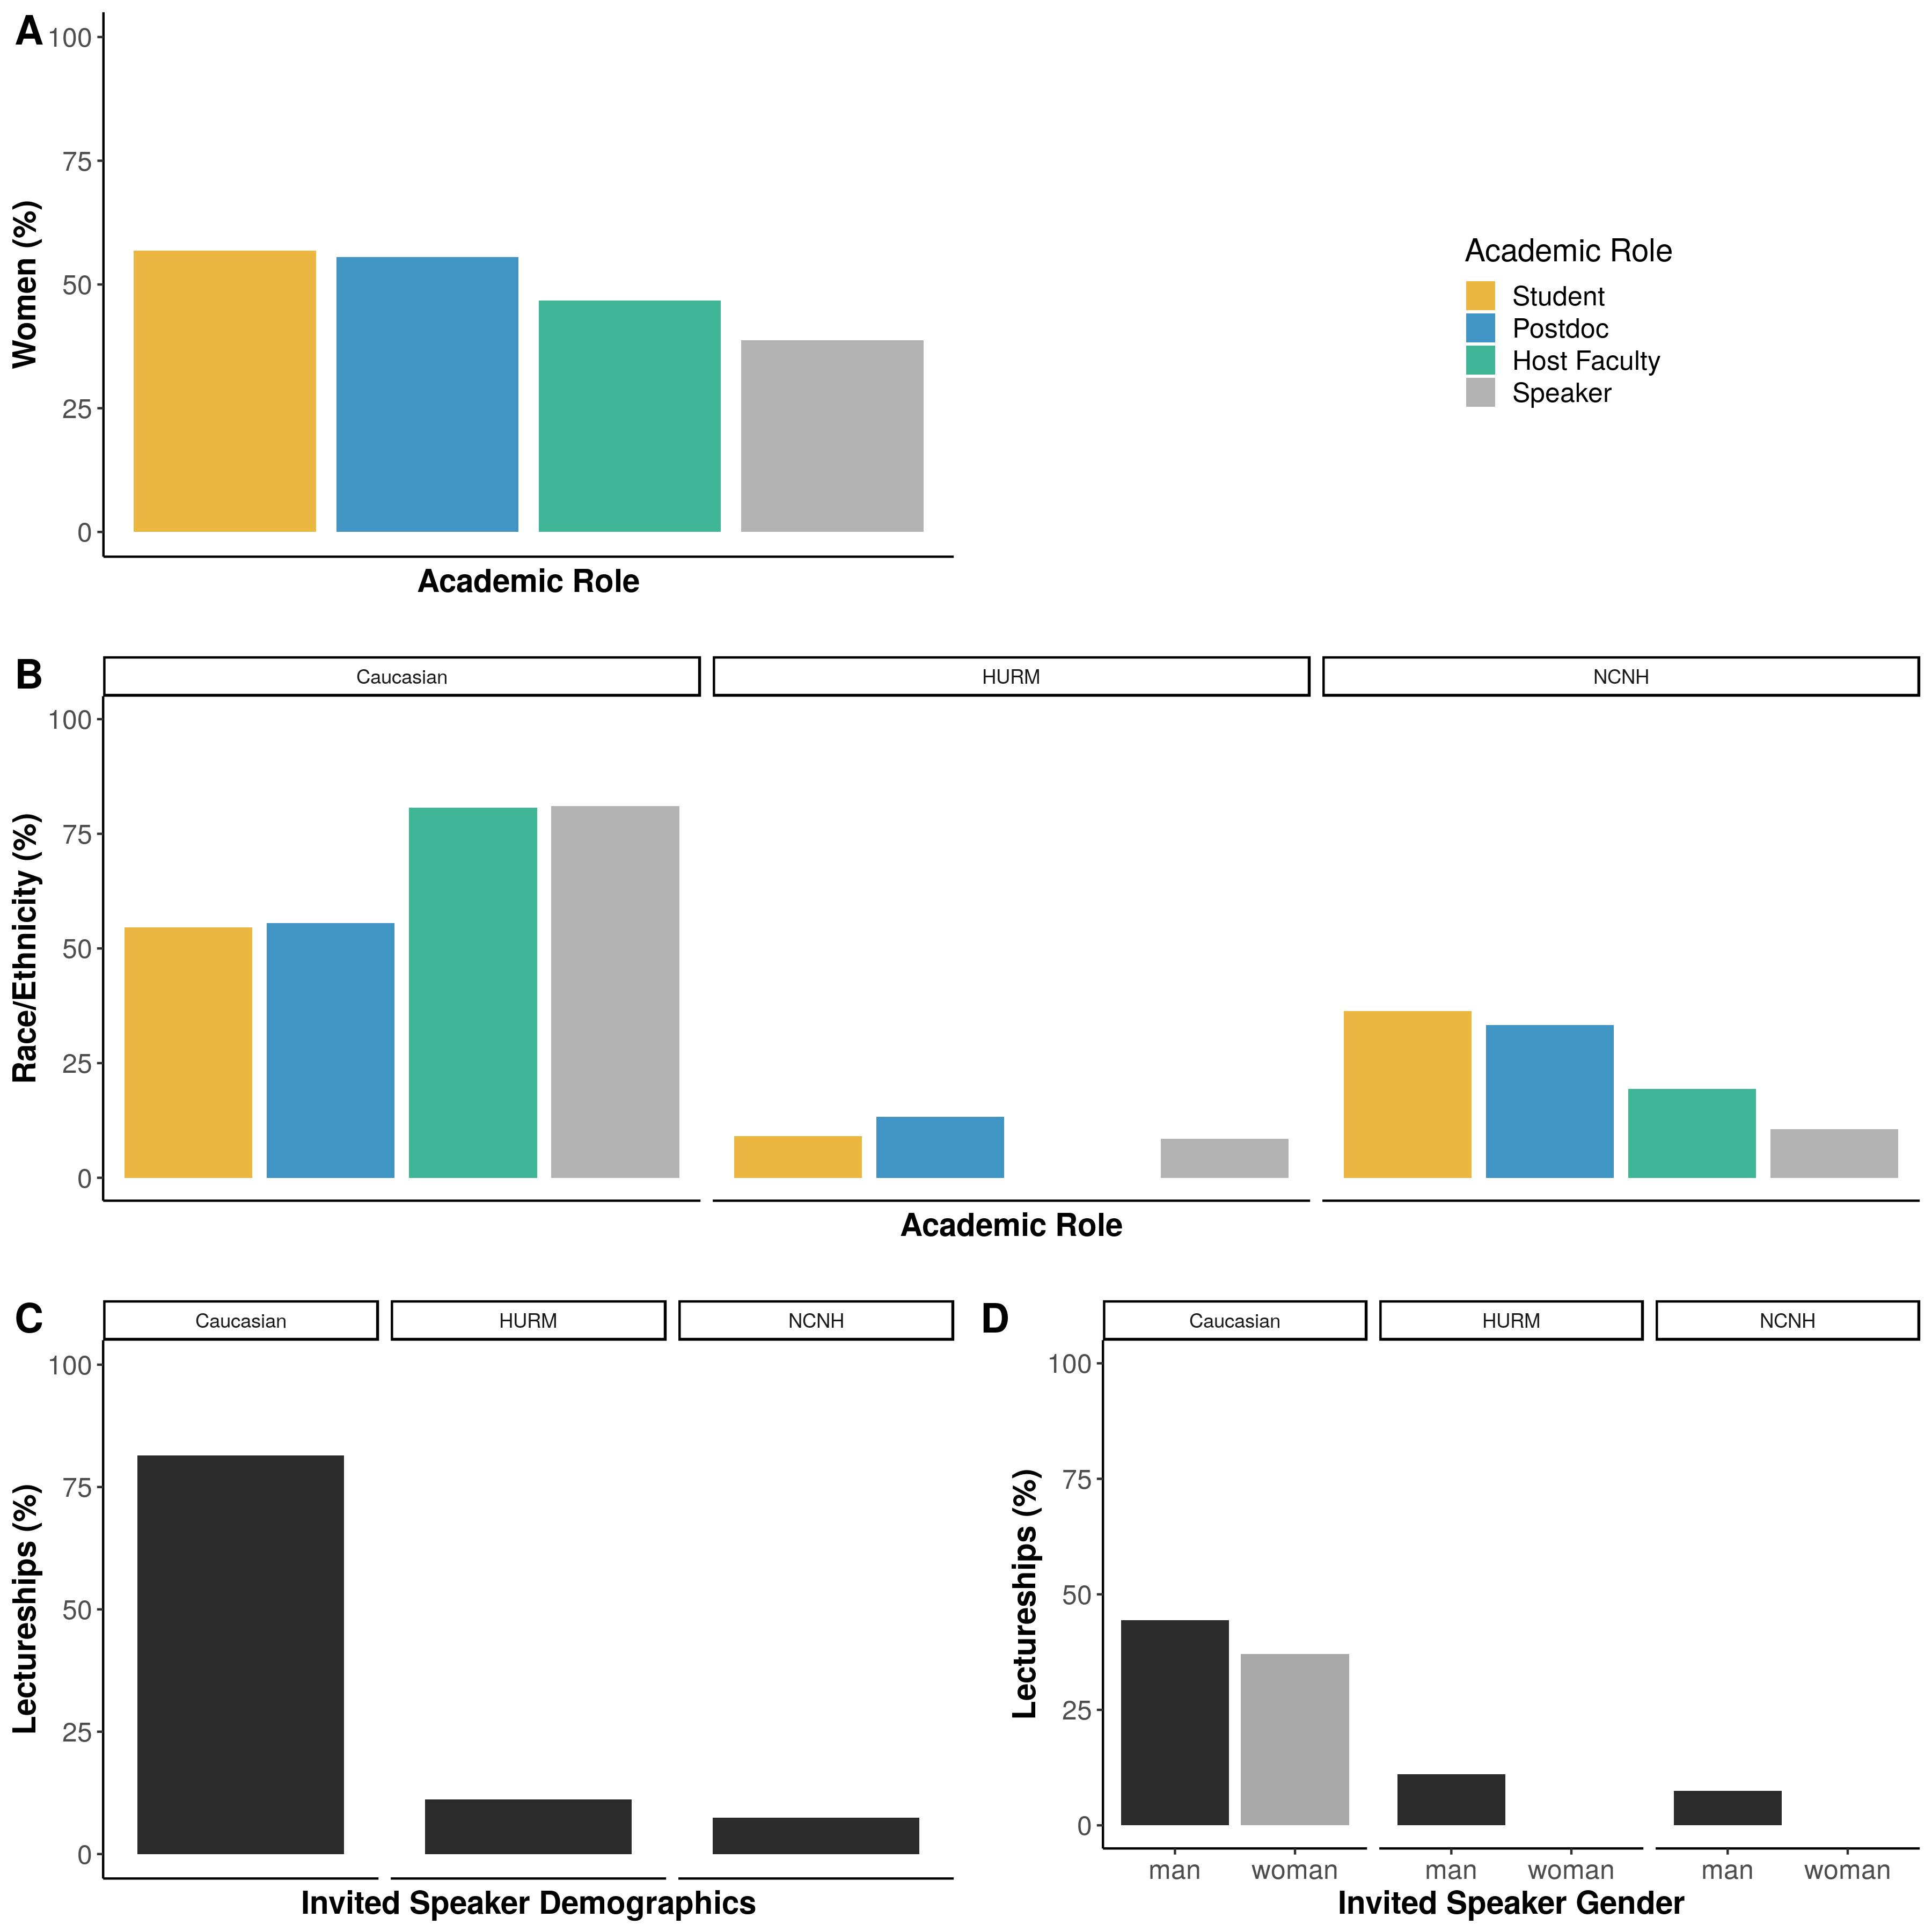
\includegraphics{Figure_1.png}
\caption{Figure 1.}
\end{figure}

\newpage

\begin{center}
\captionof{table}{List of suggestions and resources to increase invited speaker diversity.}
\small
\begin{tabular}{|l|l|l|}
\hline

\rowcolor{lightgray}
\textbf{Suggestion} & \textbf{Description} & \textbf{Resource} \\ \hline

Lab-invited speakers & \makecell[l]{Faculty members can request \\suggestions from trainees} & \\ \hline

Use a list & \makecell[l]{Many lists of scientists from \\under-represented and underserved \\groups are available} &  \makecell[l]{https://DiversifyMicrobiology.\\github.io/resources}\\ \hline

Create a list & \makecell[l]{Use the GitHub template \\ create a self-nomination list and \\resource for your field} & \makecell[l]{https://github.com/diversifymicrobiology/\\DiversifyMicrobiology.github.io} \\ \hline

Highlight the journey & \makecell[l]{Invite all speakers to spend \\a few moments describing their \\personal science journey} & \\ \hline

\end{tabular}
\end{center}

\newpage

\subsection{References}\label{references}

\hypertarget{refs}{}


\end{document}
